% SC3000 — Chapter 6: Logic and Knowledge Representation (0->100)
% No \documentclass — included by main.tex
\chapter{Logic and Knowledge Representation}\label{ch:logic}

\begin{quote}
\emph{``Logic is the calculus of reasoning.''} A knowledge-based agent separates \emph{what it knows} (a knowledge base) from \emph{how it reasons} (inference). Logic gives both a language and a guarantee: if the premises entail a sentence, a complete proof procedure will find it.
\end{quote}

\noindent\fbox{\parbox{\dimexpr\linewidth-2\fboxsep-2\fboxrule}{%
\textbf{From zero: search $\to$ knowledge.} Ch.~2--4 searched state spaces; this chapter asks how an agent \emph{represents} and \emph{derives} knowledge. We build propositional logic from truth tables, then lift it to first-order logic. No prior logic assumed.}}
\vspace{0.4em}

\section*{Learning Outcomes}
After this chapter you will be able to:
\begin{enumerate}[label=(L\arabic*)]
    \item formalise sentences in propositional and first-order logic (FOL);
    \item test entailment $KB \models \alpha$ via truth tables and convert to CNF;
    \item apply resolution, forward chaining and backward chaining;
    \item interpret FOL semantics (domains, interpretations, models) and compute unifiers;
    \item trace FOL resolution with unification and standardising apart.
\end{enumerate}

% ============================================================
\section{Propositional Logic: Syntax, Semantics, Entailment}\label{sec:prop}
A \emph{proposition} is a statement that is true or false. Propositional atoms $P,Q,R$ combine with connectives $\lnot,\land,\lor,\Rightarrow,\Leftrightarrow$. A \emph{model} $m$ assigns each atom T/F; semantics is the usual truth tables ($\lnot$, $\land$, $\lor$, $\Rightarrow\equiv\lnot P\lor Q$).

$KB \models \alpha$ (entailment) iff every model of $KB$ satisfies $\alpha$. Equivalently, $KB\land\lnot\alpha$ is unsatisfiable --- the basis for refutation.

\begin{figure}[h!]\centering
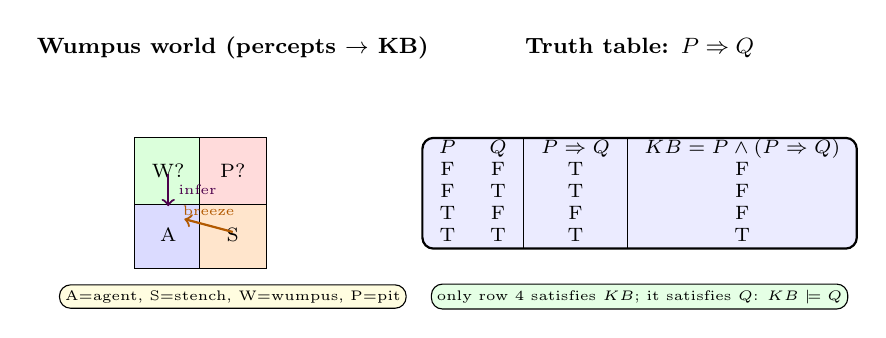
\begin{tikzpicture}[every node/.style={font=\scriptsize}, scale=0.82]
% Wumpus grid 2x2
\begin{scope}
\node[font=\footnotesize\bfseries] at (1.5,3.4) {Wumpus world (percepts $\to$ KB)};
\foreach \x in {0,1,2} \foreach \y in {0,1,2} {\draw[gray!60] (\x,\y) -- (\x,2); \draw[gray!60] (\x,\y) -- (2,\y);}
\node[draw, fill=blue!14, minimum size=0.85cm] at (0.5,0.5) {A};
\node[draw, fill=orange!20, minimum size=0.85cm] at (1.5,0.5) {S};
\node[draw, fill=green!14, minimum size=0.85cm] at (0.5,1.5) {W?};
\node[draw, fill=red!14, minimum size=0.85cm] at (1.5,1.5) {P?};
\node[font=\tiny, fill=yellow!12, draw, rounded corners, inner sep=2pt] at (1.5,-0.45) {A=agent, S=stench, W=wumpus, P=pit};
% breeze/stench percept arrows
\draw[->, thick, orange!70!black] (1.5,0.55) -- (0.75,0.75) node[midway, above, font=\tiny] {breeze};
\draw[->, thick, violet!60!black] (0.5,1.45) -- (0.5,0.95) node[midway, right, font=\tiny] {infer};
\end{scope}
% Truth table
\begin{scope}[xshift=6.2cm]
\node[font=\footnotesize\bfseries] at (1.6,3.4) {Truth table: $P\Rightarrow Q$};
\node[draw, thick, fill=blue!8, rounded corners, inner sep=0pt] (tbl) at (1.6,1.15) {
\begin{tabular}{cc|c|c}
\toprule $P$ & $Q$ & $P\Rightarrow Q$ & $KB=P\land(P\Rightarrow Q)$\\\midrule
F & F & T & F\\ F & T & T & F\\ T & F & F & F\\ T & T & T & T\\\bottomrule
\end{tabular}};
\node[font=\tiny, fill=green!10, draw, rounded corners, inner sep=2pt] at (1.6,-0.45) {only row 4 satisfies $KB$; it satisfies $Q$: $KB\models Q$};
\end{scope}
\end{tikzpicture}
\caption{Left: Wumpus grid --- percepts (stench, breeze) enter $KB$ as sentences. Right: truth table shows entailment $ \{P, P\Rightarrow Q\}\models Q$; only the $KB$-models matter.}
\label{fig:wumpus-truth}
\end{figure}

CNF (conjunctive normal form) is a conjunction of clauses, each a disjunction of literals. Every sentence converts via: eliminate $\Leftrightarrow,\Rightarrow$, push $\lnot$ inward (De Morgan), distribute $\lor$ over $\land$.

% ============================================================
\section{Inference: Resolution, Forward and Backward Chaining}\label{sec:resolution}
The \emph{resolution rule} on clauses $( \ell\lor C_1)$ and $(\lnot\ell\lor C_2)$ derives $(C_1\lor C_2)$ (the resolvent). Resolution is sound and \emph{refutation-complete} for CNF: to prove $KB\models\alpha$, add $\lnot\alpha$ to $KB$, convert to CNF, and derive the empty clause $\Box$.

Forward chaining (FC) fires \emph{definite clauses} ($p_1\land\dots\land p_k\Rightarrow q$) whenever premises are known, adding $q$ until fixpoint --- data-driven, $O(n)$ for Horn KBs, complete for Horn. Backward chaining (BC) is goal-driven: to prove $q$, prove its premises recursively (depth-first, as in Prolog), with memoisation.

\begin{figure}[h!]\centering
\begin{tikzpicture}[every node/.style={font=\scriptsize},
  cl/.style={draw, thick, rounded corners, align=center, minimum width=2.1cm, minimum height=0.62cm},
  res/.style={font=\tiny, fill=orange!12, draw=orange!40!black, rounded corners}]
\node[cl, fill=blue!12] (c1) at (0,2.6) {$C_1\!:\;P\lor Q$};
\node[cl, fill=blue!12] (c2) at (4,2.6) {$C_2\!:\;\lnot P\lor R$};
\node[cl, fill=green!14] (c3) at (2,1.4) {$C_4\!:\;Q\lor R$};
\node[cl, fill=violet!12] (c4) at (6.5,1.4) {$C_3\!:\;\lnot R$};
\node[cl, fill=orange!18] (c5) at (4.2,0.15) {$C_5\!:\;Q$};
\node[cl, fill=red!14] (c6) at (4.2,-0.95) {$\Box$ (empty)};
\node[cl, fill=gray!12, dashed] (c7) at (1.8,-0.95) {$\lnot Q$};
\draw[->, thick, blue!60!black] (c1) -- (c3); \draw[->, thick, blue!60!black] (c2) -- (c3);
\draw[->, thick, violet!60!black] (c3) -- (c5); \draw[->, thick, violet!60!black] (c4) -- (c5);
\draw[->, thick, red!60!black] (c5) -- (c6); \draw[->, thick, red!60!black, dashed] (c7) -- (c6);
\node[res] at (2,2.05) {resolve on $P$}; \node[res] at (5.6,0.78) {resolve on $R$}; \node[res] at (2.9,-0.42) {resolve on $Q$};
\node[font=\tiny, fill=yellow!10, draw, rounded corners, inner sep=2pt, align=left] at (0.2,0.15) {KB: $C_1,C_2,C_3$\\query $\lnot Q\Rightarrow\Box$};
\end{tikzpicture}
\caption{Resolution proof tree (refutation). Adding $\lnot Q$ to $KB=\{P\lor Q,\;\lnot P\lor R,\;\lnot R\}$ yields $\Box$; hence $KB\models Q$. Coloured levels show successive resolvents.}
\label{fig:resolution-tree}
\end{figure}

\begin{lstlisting}[language=Python, caption={Propositional resolution (refutation) on CNF clauses}, label={lst:prop-res}]
def resolve(ci, cj):
    """ci, cj are frozensets of literals like 'P' or '~P'. Yield resolvents."""
    for lit in ci:
        comp = lit[1:] if lit.startswith("~") else "~"+lit
        if comp in cj:
            resolvent = (ci - {lit}) | (cj - {comp})
            # tautology check: contains both x and ~x
            if not any((l[1:] if l.startswith("~") else "~"+l) in resolvent for l in resolvent):
                yield frozenset(resolvent)

def pl_resolution(kb, query):
    """kb: list of clauses; query: literal. Returns True if kb |= query."""
    neg = "~" + query if not query.startswith("~") else query[1:]
    clauses = set(kb) | {frozenset([neg])}   # add negated query
    new = set()
    while True:
        for ci in list(clauses):
            for cj in list(clauses):
                if ci is cj: continue
                for r in resolve(ci, cj):
                    if len(r) == 0: return True   # empty clause
                    new.add(r)
        if new.issubset(clauses): return False
        clauses |= new

# KB = {P v Q, ~P v R, ~R}  entails Q ?
kb = [frozenset({"P","Q"}), frozenset({"~P","R"}), frozenset({"~R"})]
print(pl_resolution(kb, "Q"))  # True
\end{lstlisting}

% ============================================================
\section{First-Order Logic: Syntax, Semantics, Unification}\label{sec:fol}
Propositional logic cannot say ``every wumpus is smelly'' without enumerating. FOL adds \emph{terms} (constants, variables, functions), \emph{predicates}, \emph{quantifiers} $\forall,\exists$, and equality.

\begin{definition}[FOL sentence]
Terms $t::=c\mid x\mid f(t_1,\dots,t_n)$; atoms $P(t_1,\dots,t_n)$; sentences $\varphi::= \text{atom}\mid\lnot\varphi\mid\varphi\land\varphi\mid\varphi\lor\varphi\mid\varphi\Rightarrow\varphi\mid\forall x\,\varphi\mid\exists x\,\varphi$.
\end{definition}

Semantics: an \emph{interpretation} $\mathcal{I}=(D,\cdot^{\mathcal{I}})$ has domain $D\neq\emptyset$ mapping each constant to $D$, function to $D^n\to D$, predicate to a relation on $D$. $\forall x\,\varphi$ holds iff $\varphi$ holds for every $d\in D$ (with $x\mapsto d$).

\emph{Unification} finds a substitution $\theta=\{x_1/t_1,\dots\}$ making two literals identical: $\textsc{Unify}(P(x,f(a)),P(b,y))$ needs $\{x/b,\;y/f(a)\}$. The \emph{most general unifier} (MGU) is unique up to renaming; occur-check ($x$ in $t$) prevents unsound cycles.

\begin{figure}[h!]\centering
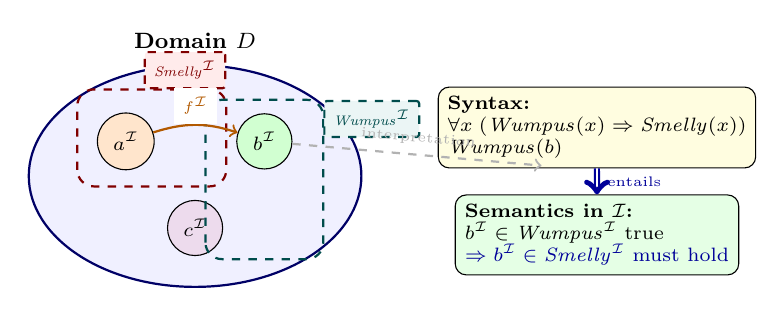
\begin{tikzpicture}[every node/.style={font=\scriptsize}, scale=0.88]
% Domain bubble
\draw[thick, fill=blue!6, draw=blue!40!black, rounded corners=8pt] (0,0) ellipse (2.4 and 1.6);
\node[font=\footnotesize\bfseries, fill=white, rounded corners=2pt, inner sep=2pt] at (0,1.95) {Domain $D$};
\node[circle, draw, fill=orange!20, minimum size=7mm] (a) at (-1.0,0.5) {$a^{\mathcal I}$};
\node[circle, draw, fill=green!18, minimum size=7mm] (b) at (1.0,0.5) {$b^{\mathcal I}$};
\node[circle, draw, fill=violet!14, minimum size=7mm] (c) at (0,-0.75) {$c^{\mathcal I}$};
% Predicates as regions
\draw[thick, red!50!black, dashed, rounded corners=6pt] (-1.7,-0.15) rectangle (0.45,1.25) node[above left, font=\tiny, fill=red!8, draw, rounded corners=1pt] {$\mathit{Smelly}^{\mathcal I}$};
\draw[thick, teal!60!black, dashed, rounded corners=6pt] (0.15,-1.2) rectangle (1.85,1.1) node[below right, font=\tiny, fill=teal!8, draw, rounded corners=1pt] {$\mathit{Wumpus}^{\mathcal I}$};
% Function arrow
\draw[->, thick, orange!70!black, bend left=18] (a) to node[midway, above, font=\tiny, fill=white] {$f^{\mathcal I}$} (b);
% Syntax side
\node[draw, fill=yellow!12, rounded corners, align=left, minimum width=3.6cm] (syn) at (5.8,0.7) {\textbf{Syntax:}\\$\forall x\;(\mathit{Wumpus}(x)\Rightarrow\mathit{Smelly}(x))$\\$ \mathit{Wumpus}(b)$};
\node[draw, fill=green!10, rounded corners, align=left, minimum width=3.6cm] (sem) at (5.8,-0.85) {\textbf{Semantics in $\mathcal I$:}\\$b^{\mathcal I}\in\mathit{Wumpus}^{\mathcal I}$ true\\\color{blue!60!black}$\Rightarrow b^{\mathcal I}\in\mathit{Smelly}^{\mathcal I}$ must hold};
\draw[->, thick, blue!60!black, double] (syn) -- (sem) node[midway, right, font=\tiny] {entails};
\draw[->, thick, gray!60, dashed] (b) -- (5.0,0.15) node[midway, above, sloped, font=\tiny] {interpretation};
\end{tikzpicture}
\caption{FOL semantics: syntax maps into a domain $D$ via $\mathcal I$. Predicates are relations (dashed regions); functions map elements. The sentence $\forall x(W(x)\Rightarrow S(x))$ constrains every element of $D$.}
\label{fig:fol-semantics}
\end{figure}

FOL resolution lifts propositional resolution with unification. Clauses are universally quantified disjunctions; variables are \emph{standardised apart} (renamed) before resolving. From $\{\lnot P(x)\lor Q(x),\;P(a)\}$ with $\theta=\{x/a\}$ derive $Q(a)$.

\begin{lstlisting}[language=Python, caption={FOL unification (MGU with occur-check)}, label={lst:fol-unify}]
def unify(x, y, theta=None):
    """Robinson unification. Terms are str vars ('?x') or [fun, args...]. Returns dict or None."""
    if theta is None: theta = {}
    if theta is None: return None
    if x == y: return theta
    if isinstance(x, str) and x.startswith("?"): return unify_var(x, y, theta)
    if isinstance(y, str) and y.startswith("?"): return unify_var(y, x, theta)
    if isinstance(x, list) and isinstance(y, list):
        if x[0] != y[0] or len(x) != len(y): return None
        for xi, yi in zip(x[1:], y[1:]):
            theta = unify(xi, yi, theta)
            if theta is None: return None
        return theta
    return None

def unify_var(var, x, theta):
    if var in theta: return unify(theta[var], x, theta)
    if isinstance(x, str) and x in theta: return unify(var, theta[x], theta)
    if occurs(var, x, theta): return None  # occur-check
    theta = dict(theta); theta[var] = x; return theta

def occurs(var, x, theta):
    if x == var: return True
    if isinstance(x, list): return any(occurs(var, a, theta) for a in x[1:])
    if isinstance(x, str) and x in theta: return occurs(var, theta[x], theta)
    return False

# e.g. Knows(?x, f(?y))  ~  Knows(John, f(Mary))
print(unify(["Knows","?x",["f","?y"]], ["Knows","John",["f","Mary"]]))
# {'?x': 'John', '?y': 'Mary'}
print(unify("?x", ["f","?x"]))  # None (occur-check)
\end{lstlisting}

\textit{FOL resolution strategy:} convert $KB\land\lnot\alpha$ to CNF (Skolemise $\exists$ to fresh functions), then repeatedly resolve complementary literals with MGU, standardising apart, until $\Box$ or saturation. It is refutation-complete for FOL; general entailment is only semi-decidable.

% ============================================================
\section{Key Takeaways}
Propositional inference reduces to CNF + resolution ($\Box$ means entailment); Horn KBs also allow linear forward/backward chaining. FOL adds expressive power via quantifiers, at the cost of undecidability --- unification + lifted resolution is the algorithmic bridge, complete for refutation but only semi-decidable in general. Design $KB$ for the task: propositional for small worlds, FOL when relations quantify over many objects.

% ============================================================
\section{Exercises}\label{sec:ch06-ex}
\begin{enumerate}[label=E6.\arabic*, leftmargin=*, itemsep=0.7em]
    \item \textbf{Entailment by truth table.} Show $\{P\Rightarrow Q,\;Q\Rightarrow R\}\models P\Rightarrow R$ using Fig.~\ref{fig:wumpus-truth} style. How many rows? Which rows are $KB$-models?
    \item \textbf{CNF + resolution.} Convert $(P\Rightarrow Q)\land(Q\Rightarrow R)\land P$ and query $R$ to CNF, then give a resolution tree (as in Fig.~\ref{fig:resolution-tree}) deriving $\Box$ from $KB\cup\{\lnot R\}$.
    \item \textbf{Chaining.} Horn KB: $P,\;P\Rightarrow Q,\;Q\land R\Rightarrow S$. Trace forward chaining from $\{P,R\}$ and backward chaining for goal $S$. Which explores fewer clauses and why?
    \item \textbf{Unification.} Find the MGU (or say why none exists) for each pair:
    \begin{itemize}[itemsep=0.15em]
        \item $P(?x, f(?x))$ vs.\ $P(a, f(b))$;
        \item $P(?x, ?y)$ vs.\ $P(f(?y), b)$;
        \item $Knows(?x,?x)$ vs.\ $Knows(John, Mary)$,
    \end{itemize}
    and explain any occur-check failure above.
    \item \textbf{FOL resolution.} From $\forall x(W(x)\Rightarrow S(x))$ and $W(b)$, prove $S(b)$ by FOL resolution: Skolemise, clausify, standardise apart, unify, and show the tree ending in $\Box$ (use Fig.~\ref{fig:fol-semantics} interpretation to argue soundness).
\end{enumerate}
% End of Chapter 6
